\section{Hi-C}

\begin{frame}[c]{High-Throughput 3C (Hi-C)}
    \normalsize
    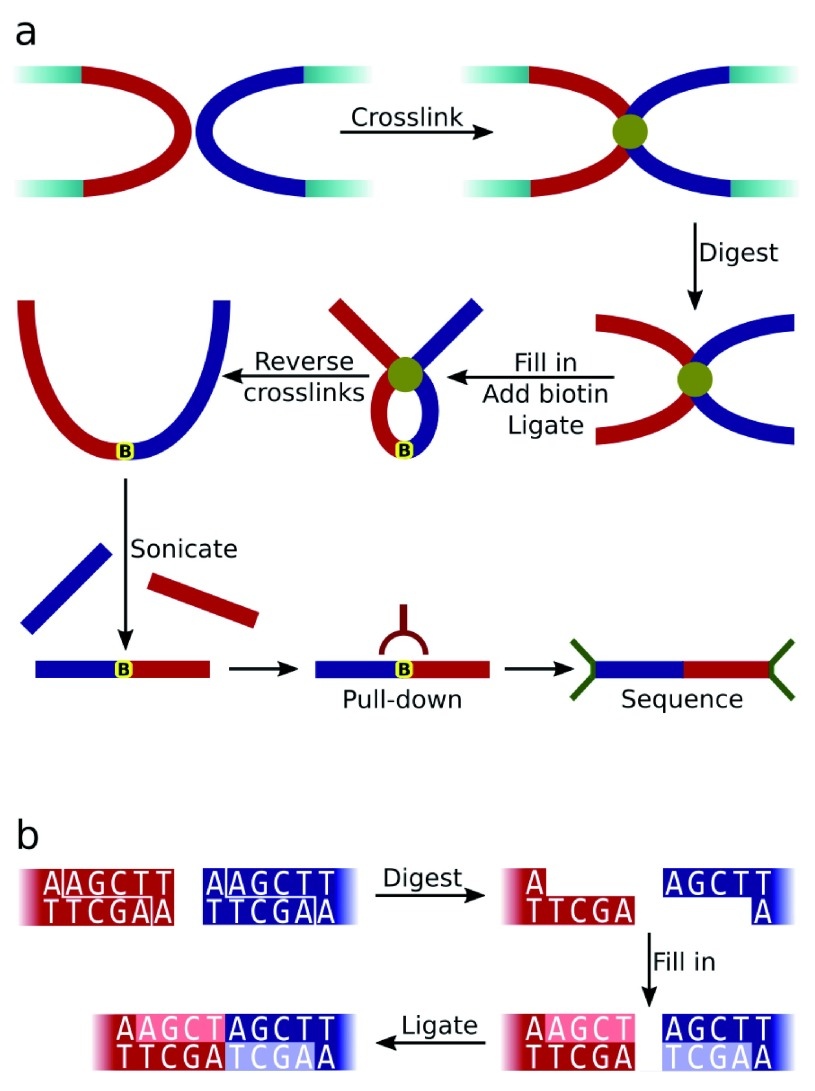
\includegraphics[scale=2.4, trim=0 40 0 6, clip]{f1000research-4-7903-g0000} \\
    Image adapted from \cite{wingett2015hicup}.
\end{frame}

\begin{frame}[c]{High-Throughput 3C (Hi-C)}
    Several biases:
    \begin{itemize}[<+(1)->]
        \item Some regions are easier labeled with biotin than others
        \item PCR artifacts \cite{wingett2015hicup}
        \item Sequencing itself has multiple biases \cite{aird2011analyzing}
        \item Where to map multiple/unclear reads
    \end{itemize}
    % \only<2>{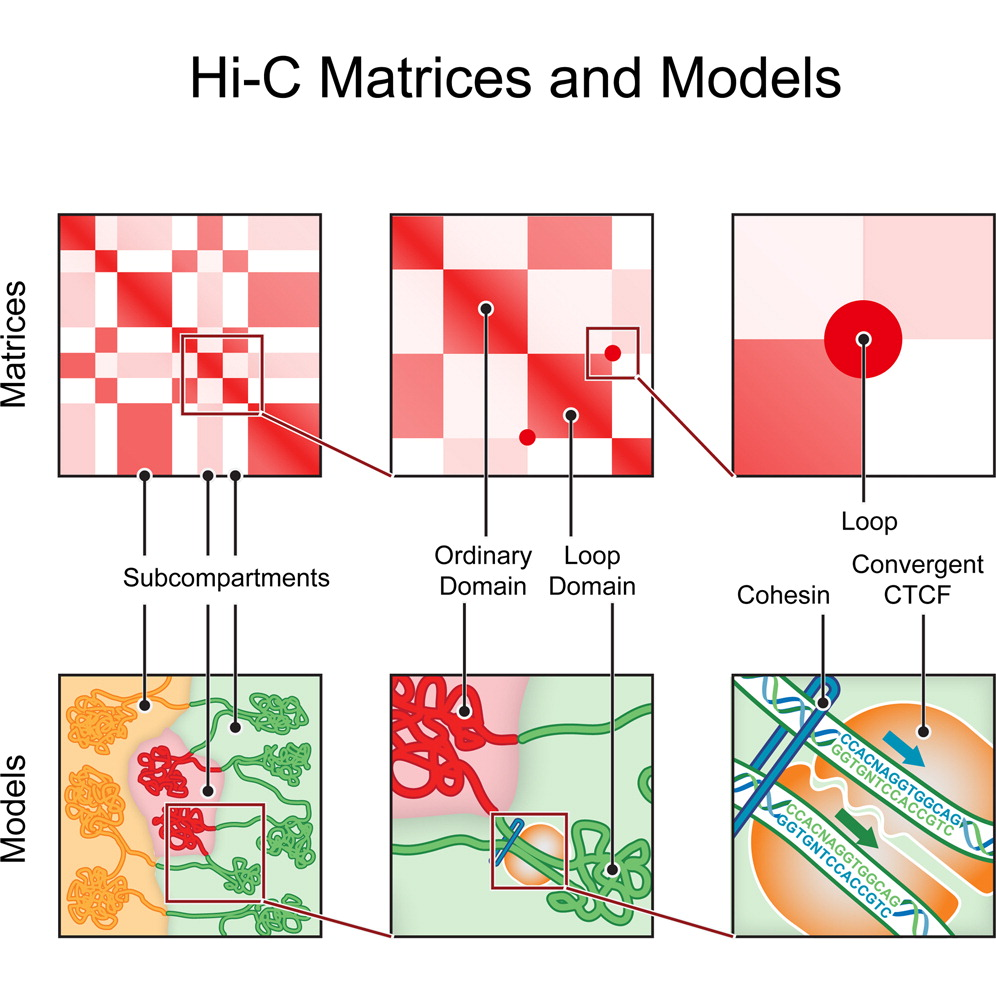
\includegraphics[scale=1.5, trim=0 0 82 130,clip]{HiCMatricesModels} \\
    % Image adapted from \cite{rao20143d}.}
    % Biases for each step:
    %
    % - Some regions do easier biotin labeling than others
    % - PCR artifacts are included
    % - Sequencing itself has multiple biases
    % - Where to map multiple/unclear reads ?
    % - differing chromatin states
    % - more ...

\end{frame}

% \begin{frame}[c]% {Chromosome Conformation Technologies}
%     \normalsize
%     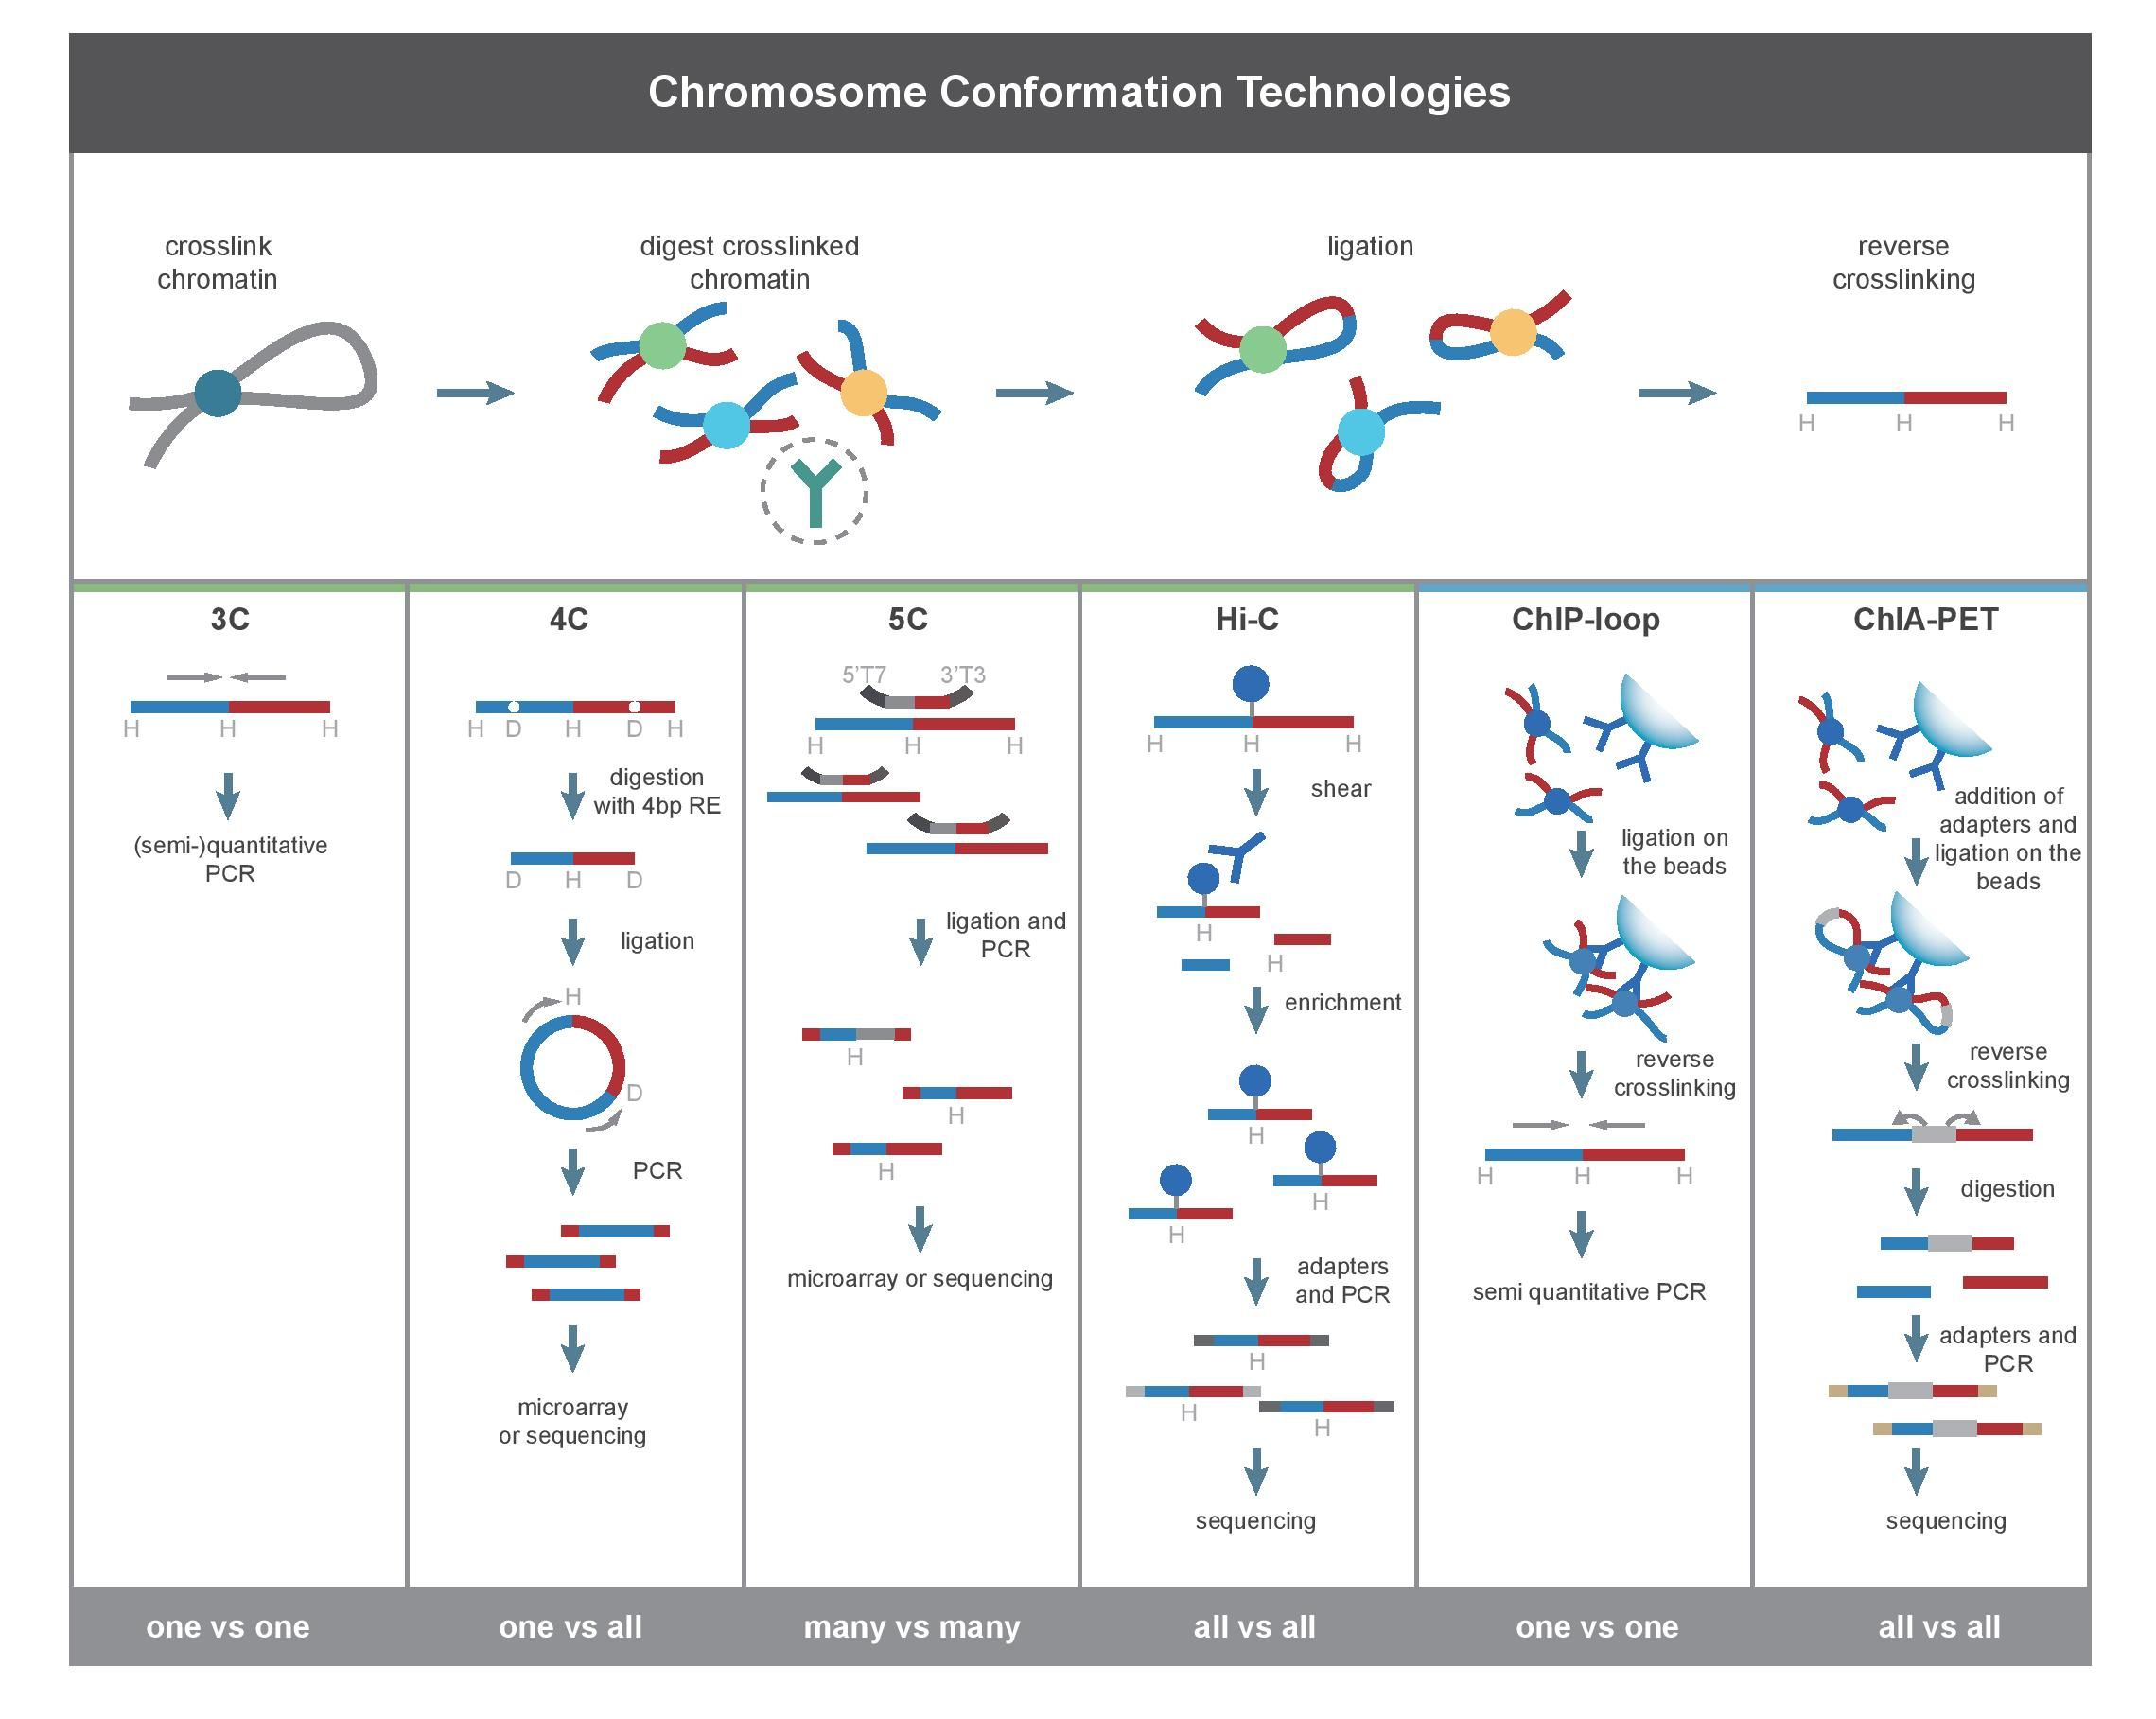
\includegraphics[scale=0.55]{Chromosome_conformation_techniques} \\
%     Image from \cite{Li2014}.
% \end{frame}


% Make introduction of Hi-C with focus to potential biases


\begin{frame}[c]{HiCExplorer}
    \large
    Helpful tools, especially for:
    \begin{itemize}[<+(1)->]
        \item Data correction
        \item Analysis
        \item Visualization
    \end{itemize}
\end{frame}


% \begin{frame}[c]{HiCExplorer}
%     \normalsize
%     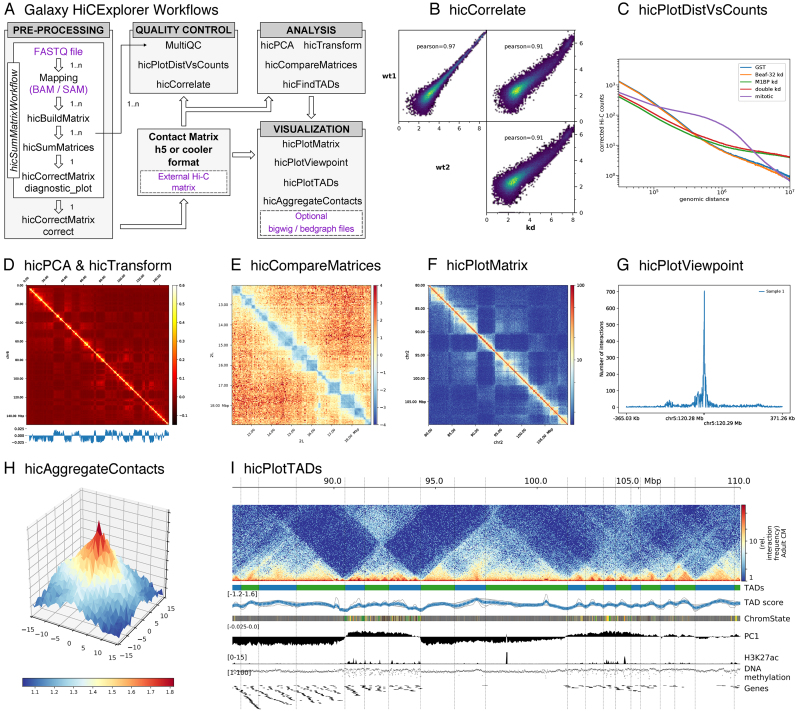
\includegraphics[scale=2.5,trim=37 0 0 45,clip]{HiCExplorer} \\
%     Image adapted from \cite{wolff2018galaxy}.
% \end{frame}


